%%%%%%%%%%%%%%%%%%%%%%%%%%%%%%%%%%%%%%%%%%%%%%%%%%%%%
%%% Task 2 %%%%%%%%%%%%%%%%%%%%%%%%%%%%%%%%%%%%%%%%%%
%%%%%%%%%%%%%%%%%%%%%%%%%%%%%%%%%%%%%%%%%%%%%%%%%%%%%
\task{Separately excited DC machine}

%%%%%%%%%%%%%%%%%%%%%%%%%%%%%%%%%%%%%%%%%%%%%%
\taskGerman{Fremderregte Gleichstrommaschine}
% Oliver
% Fremderregte DC-Maschine in Anlehnung an Aufgabe 4.16 Aufgabensammlung EMA Binder (Teil2)
% ggf. ergänzt um transiente Reaktion

\begin{table}[htb]
    \caption{DC machine parameters.}
    \centering
    \begin{tabular}{lll}\toprule
    Symbol  & Description       & Values \\
    \midrule
    $U_{\mathrm{a,n}}$    & Nominal armature voltage           & $\SI{230}{\volt}$ \\
    $I_{\mathrm{a,n}}$    & Nominal armature current           & $\SI{22}{\ampere}$ \\
    $U_{\mathrm{f,n}}$    & Nominal field voltage           & $\SI{230}{\volt}$ \\
    $I_{\mathrm{f,n}}$    & Nominal field current           & $\SI{0.5}{\ampere}$ \\
    $P_{\mathrm{n}}$    & Nominal power             & $\SI{4.5}{\kilo\watt}$ \\
    $n_{\mathrm{n}}$    & Nominal speed             & $\SI[fraction-function=\nicefrac]{1440}{\per\minute}$ \\
    $n_{0}$    & No-load speed             & $\SI[fraction-function=\nicefrac]{1615}{\per\minute}$ \\
    $p$     & Pole pair number              & 2 \\
    $L_\mathrm{a}$ & Armature inductance & \SI{6.92}{\henry}\\
    \bottomrule
    \end{tabular}
    \label{tab:characteristicsIM_task3}
\end{table}


\subtask{Determine the torque $T_\mathrm{n}$ and the efficiency $\eta_\mathrm{n}$ at the nominal operating point.}{2}

\subtaskGerman{Bestimmen Sie das Drehmoment $T_\mathrm{n}$ sowie den Wirkungsgrad $\eta_\mathrm{n}$ im Nennarbeitspunkt.}

\begin{solutionblock}
The nominal torque is
$$
T_\mathrm{n} = \frac{P_\mathrm{n}}{\omega_\mathrm{n}} = \frac{P_\mathrm{n}}{n_\mathrm{n}} \SI{\frac{60}{2\pi}}{\second\per\minute} = \frac{\SI{4.5}{\kilo\watt}}{\SI{1440}{\per\minute}} \SI{\frac{60}{2\pi}}{\second\per\minute} = \SI{29.84}{\newton\meter}.
$$
The electrical input power is
$$
P_\mathrm{el,n} = U_\mathrm{a,n} I_\mathrm{a,n} + U_\mathrm{f,n} I_\mathrm{f,n} = \SI{5.06}{\kilo\watt} + \SI{115}{\watt} = \SI{5.18}{\kilo\watt}.
$$
The resulting efficiency yields
$$
\eta_\mathrm{n} = \frac{P_\mathrm{n}}{P_\mathrm{el,n}} = \SI{86.87}{\percent}.
$$
\end{solutionblock}

\subtask{How large are the armature resistance $R_\mathrm{a}$ and the resulting armature losses $P_\mathrm{l,a}$ at the nominal operation neglecting iron and mechanical losses?}{2}%
\begin{hintblock}
if and if only you are not able to solve this task, use $R_\mathrm{a} = \SI{3.2}{\ohm}$ and $\psi'_\mathrm{f} = \SI{1.1}{\volt\second}$ as a substitute result for the subsequent tasks.
\end{hintblock}

\subtaskGerman{Wie groß ist der Ankerwiderstand $R_\mathrm{a}$ und wie hoch sind die resultierenden Ankerverluste $P_\mathrm{l,a}$ im Nennarbeitspunkt unter Vernachlässigung von Eisenverlusten und mechanischen Verlusten?}%
\begin{germanhintblock}
nur für den Fall, dass Sie kein Ergebnis ermitteln können, verwenden Sie $R_\mathrm{a} = \SI{3,2}{\ohm}$ und $\psi'_\mathrm{f} =$ \SI{1,1}{\volt\second} für die nachfolgenden Aufgaben.
\end{germanhintblock}


\begin{solutionblock}
    In the no-load case, the entire armature voltage is identical to the induced voltage given a constant field excitation
    $$
    U_\mathrm{i,0} = U_\mathrm{a,n} = \omega_0 \psi'_\mathrm{f}. 
    $$
    Hence, the effective field flux linkage is
    $$
    \psi'_\mathrm{f} = \frac{U_\mathrm{a,n}}{\omega_0} = \frac{\SI{230}{\volt}}{\SI{1615}{\per\minute} \cdot \SI{\frac{2\pi}{60}}{\minute\per\second}} = \SI{1.36}{\volt\second}.
    $$
    At nominal (loaded) operation, the armature voltage equation is
    $$
    U_\mathrm{a,n} = R_\mathrm{a}I_\mathrm{a,n} + \omega_\mathrm{n} \psi'_\mathrm{f}
    $$
    delivering the armature resistance
    $$
    R_\mathrm{a} = \frac{U_\mathrm{a,n} - \omega_\mathrm{n} \psi'_\mathrm{f}}{I_\mathrm{a,n}} = \frac{\SI{230}{\volt} - \SI{1440}{\per\minute} \cdot \SI{\frac{2\pi}{60}}{\minute\per\second} \cdot \SI{1.36}{\volt\second}}{\SI{22}{\ampere}} = \SI{1.13}{\ohm}.
    $$
    The nominal armature losses result in:
    $$
     P_\mathrm{l,a} = R_\mathrm{a} I^2_\mathrm{a,n} = \SI{1.13}{\ohm} \cdot \SI{484}{\ampere\squared} = \SI{546.92}{\watt}.
    $$
\end{solutionblock}

\subtask{For a new operating point at $n=\SI[fraction-function=\nicefrac]{900}{\per\minute}$, a torque of $T=\SI{20}{\newton\meter}$ is to be achieved. For this purpose, an additional dropping resistor $R_\mathrm{d}$ is introduced into the armature circuit. Determine its required resistance value.}{2}
\begin{hintblock}
if and if only you are not able to solve this task, use $R_\mathrm{d} = \SI{4.2}{\ohm}$ as a substitute result for the subsequent tasks.
\end{hintblock}
\subtaskGerman{Für einen neuen Betriebspunkt bei $n=\SI[fraction-function=\nicefrac]{900}{\per\minute}$ soll ein Drehmoment von $T=\SI{20}{\newton\meter}$ erzielt werden. Hierzu wird ein Vorwiderstand $R_\mathrm{d}$ in den Ankerkreis eingebracht. Bestimmen Sie dessen notwendigen Widerstandswert.}
\begin{germanhintblock}
nur für den Fall, dass Sie kein Ergebnis ermitteln können, verwenden Sie $R_\mathrm{d} = \SI{4,2}{\ohm}$ für die nachfolgenden Aufgaben.
\end{germanhintblock}

\begin{solutionblock}
    Since the field winding is not affected by the dropping resistor or speed change, the excitation $\psi'_\mathrm{f}$ remains as previously calculated. Based on the torque equation, one can calculate the required armature current:
    $$
    T = \psi'_\mathrm{f} I_\mathrm{a} \quad \Leftrightarrow \quad I_\mathrm{a} = \frac{T}{\psi'_\mathrm{f}} = \frac{\SI{20}{\newton\meter}}{\SI{1.36}{\volt\second}} = \SI{14.71}{\ampere}.
    $$
    The armature ohmic voltage drop (incl. dropping resistor) for the new operation point is
    $$
    U_\mathrm{R} = U_\mathrm{a,n} - \omega \psi'_\mathrm{f} = \SI{230}{\volt} - \SI{900}{\per\minute} \cdot \SI{\frac{2\pi}{60}}{\minute\per\second} \SI{1.36}{\volt\second} = \SI{101.82}{\volt} \stackrel{!}{=} I_\mathrm{a}(R_\mathrm{a} + R_\mathrm{d})
    $$
    delivering the required dropping resistance of
    $$
    R_\mathrm{d} = \frac{U_\mathrm{R}}{I_\mathrm{a}} - R_\mathrm{a} = \frac{\SI{101.82}{\volt}}{\SI{14.71}{\ampere}} - \SI{1.13}{\ohm} = \SI{5.79}{\ohm}.
    $$
\end{solutionblock}

\subtask{Determine the efficiency at this new operating point. What are the alternatives to introducing a dropping resistor to achieve the required torque at the new operating point and why should these alternatives be considered?}{2}
\subtaskGerman{Bestimmen Sie den Wirkungsgrad in diesem neuen Arbeitspunkt. Welche Alternativen zum Einbringen eines Vorwiderstands, um das geforderte Drehmoment im neuen Arbeitspunkt zu erzielen, bestehen und warum sollte man diese Alternativen in Betracht ziehen?}

\begin{solutionblock}
    The new total input power is
    $$
P_\mathrm{el} = U_\mathrm{a,n} I_\mathrm{a} + U_\mathrm{f,n} I_\mathrm{f,n} = \SI{3.38}{\kilo\watt} + \SI{115}{\watt} = \SI{3.50}{\kilo\watt}
$$
 and the new mechanical output power is
 $$
 P = T n \SI{\frac{2\pi}{60}}{\minute\per\second} = \SI{20}{\newton\meter} \cdot \SI{900}{\per\minute} \cdot\SI{\frac{2\pi}{60}}{\minute\per\second} = \SI{1.88}{\kilo\watt}
 $$
 resulting in the new efficiency
 $$
 \eta = \frac{P}{P_\mathrm{el}} = \frac{\SI{1.88}{\kilo\watt}}{\SI{3.50}{\kilo\watt}} = \SI{53.71}{\percent}.
 $$
 Possible alternatives are:
 \begin{itemize}
     \item Decreasing the armature voltage supply $U_\mathrm{a}$ (e.g., via a buck converter),
     \item Increasing the field excitation $\psi'_\mathrm{f}$ (e.g., via a boost converter in field circuit).
 \end{itemize}
From above's calculation a significant decrease of the machine efficiency due to the dropping resistor can be observed, which motivates the alternatives (since they typically add only little addition losses).
\end{solutionblock}

\subtask{Now the transient response of a machine supply fault should be investigated: calculate $i_\mathrm{a}(t)$ for $t \geq 0$ assuming $i_\mathrm{a}(t=0) = I_\mathrm{a,n}$ and $u_\mathrm{a}(t)=0$ for $t \geq 0$ (short circuit of armature voltage supply). Assume further that the machine speed $n(t)=n_\mathrm{n}$ for $t \geq 0$ remains constant and that the field winding is unaffected by the armature supply fault, i.e., delivering nominal excitation.}{2}
\subtaskGerman{Nun soll die transiente Reaktion bei einem Fehler in der Ankerspeisung untersucht werden: Berechnen Sie $i_\mathrm{a}(t)$ für $t \geq 0$ unter der Annahme, dass $i_\mathrm{a}(t=0) = I_\mathrm{a,n}$ und $u_\mathrm{a}(t)=0$ für $t \geq 0$ (Kurzschluss der Ankerspannungsversorgung) gilt. Nehmen Sie weiter an, dass die Maschinendrehzahl $n(t)=n_\mathrm{n}$ für $t \geq 0$ konstant bleibt und dass die Erregerwicklung von der Störung der Ankers unbeeinflusst im Nennbetrieb bleibt.}

\begin{solutionblock}
    Starting point for solving the task is the armature current ODE:
    \begin{align*}
    \frac{\mathrm{d}}{\mathrm{d} t} i_\mathrm{a}(t) &= \frac{1}{L_\mathrm{a}}\left(u_\mathrm{a}(t) - R_\mathrm{a} i_\mathrm{a}(t) - u_\mathrm{i}(t)  \right)\\ & = \frac{1}{L_\mathrm{a}}\left(- R' i_\mathrm{a}(t) - u_\mathrm{i}  \right)
    \end{align*}
    with $R' = R_\mathrm{a} + R_\mathrm{d}$.  Based on the subtask's assumptions the armature voltage at its terminals is zero $u_\mathrm{a}(t)=0$ and the induced voltage is a constant $u_\mathrm{i}(t) = u_\mathrm{i}$.  This results in a simple scalar, nonhomogeneous ODE. The homogeneous solution candidate is $x_\mathrm{h}(t) = e^{\lambda t}$, which delivers
    \begin{align*}
    \lambda e^{\lambda t} &= - \frac{R'}{L_\mathrm{a}} e^{\lambda t}
    \\
    \Leftrightarrow \qquad \lambda &=- \frac{R'}{L_\mathrm{a}} = \frac{1}{\tau_\mathrm{a}}
    \end{align*}
    when inserted into the homogeneous part of the ODE leading to the time constant $\tau_\mathrm{a}$. To solve the entire inhomogenous ODE we apply the variation of parameter approach using
    $$
    i_\mathrm{a}(t) = C(t)e^{\lambda t}.
    $$
    Inserting into the ODE yields
    \begin{alignat*}{3}
   &&\quad \dot{C}(t) e^{\lambda t} +  C(t) \lambda e^{\lambda t} &&&=  C(t) \lambda e^{\lambda t} - \frac{1}{L_\mathrm{a}} u_\mathrm{i} \\
    \Leftrightarrow&& \qquad \dot{C}(t) e^{\lambda t} &&&= - \frac{1}{L_\mathrm{a}} u_\mathrm{i}\\
    \Leftrightarrow&& \qquad \dot{C}(t) &&&= -\frac{1}{L_\mathrm{a}} u_\mathrm{i} e^{-\lambda t}
    \end{alignat*}
    delivering the integration result
    $$
    C(t) = \frac{u_\mathrm{i}}{L_\mathrm{a} \lambda} e^{-\lambda t} + C_0 =  -\frac{u_\mathrm{i}}{R'} e^{-\lambda t} + C_0.
    $$
    The overall solution is then
    $$
    i_\mathrm{a}(t) = C_0 e^{\lambda t} - \frac{u_\mathrm{i}}{R'} .
    $$
    The integration constant $C_0$ can be found from the initial condition
    $$
    i_\mathrm{a}(t=0) = I_\mathrm{a,n} = C_0 - \frac{u_\mathrm{i}}{R'} \quad \Leftrightarrow \quad C_0 = I_\mathrm{a,n} + \frac{u_\mathrm{i}}{R'} .
    $$
    Hence, we finally receive
    \begin{align*}
        i_\mathrm{a}(t) &= I_\mathrm{a,n} e^{\lambda t} + \frac{u_\mathrm{i}}{R'}(e^{\lambda t}-1) = I_\mathrm{a,n} e^{-\frac{R'}{L_\mathrm{a}} t} + \frac{u_\mathrm{i}}{R'}(e^{-\frac{R'}{L_\mathrm{a}} t}-1)\\
        &= \SI{22}{\ampere} \cdot e^{-t / \SI{1}{\second}} + \frac{\SI{205.08}{\volt}}{\SI{6.92}{\ohm}}(e^{-t / \SI{1}{\second}}-1)\\
        &= \SI{22}{\ampere} \cdot e^{-t / \SI{1}{\second}} + \SI{29.64}{\ampere} (e^{-t / \SI{1}{\second}}-1).
    \end{align*}
\end{solutionblock}

\subtask{Sketch the current response $i_\mathrm{a}(t)$ as a function of time $t$. Also calculate the steady-state value for $t\rightarrow \infty$.}{2}
\begin{hintblock}
    if and if only you have not solved the previous subtask, you can draw the current trajectory qualitatively to highlight the general system response characteristic for the given differential equation model. Also note, that the question addressing the steady-state armature current can be answered independently of the previous subtask.
\end{hintblock}
\subtaskGerman{Zeichnen Sie die Stromreaktion $i_\mathrm{a}(t)$ als Funktion über die Zeit $t$. Bestimmen Sie zudem den stationären Endwert für $t\rightarrow \infty$ an.}
\begin{germanhintblock}
    nur für den Fall, dass Sie für die vorherige Teilaufgabe kein Ergebnis ermitteln konnten, können Sie die Stromkurve qualitativ zeichnen, um die prinzipielle Systemantwort für das gegebene Differentialgleichungsmodell zu verdeutlichen. Beachten Sie auch, dass die Frage nach dem stationären Endwert des Ankerstroms unabhängig von der vorherigen Teilaufgabe beantwortet werden kann.
\end{germanhintblock}

\begin{solutionblock}
    The steady-state final value can be directly obtained from the ODE (without solving it): setting $\nicefrac{\mathrm{d}}{\mathrm{d}t}(i_\mathrm{a}(t))=0$ leading to
    $$
        0 = \frac{1}{L_\mathrm{a}}\left(- R' i_\mathrm{a}(t\rightarrow\infty) - u_\mathrm{i}  \right) \qquad 
        \Leftrightarrow \qquad  i_\mathrm{a}(t\rightarrow\infty) = - \frac{u_\mathrm{i}}{R'} = \SI{-29.64}{\ampere}. 
    $$
    \begin{solutionfigure}[ht]
    \centering
    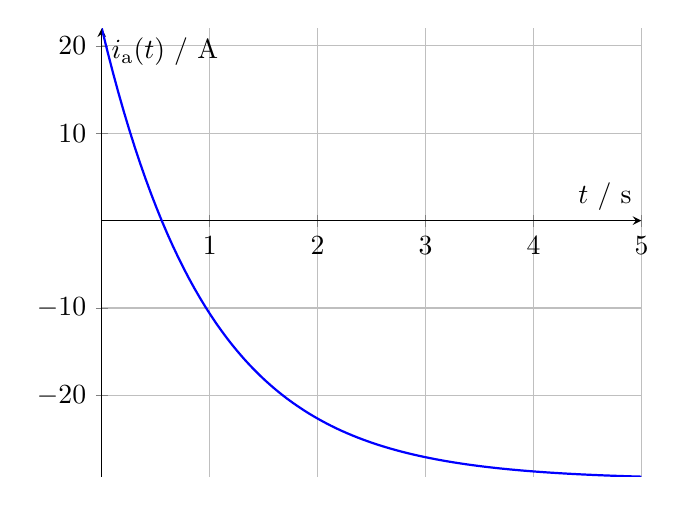
\begin{tikzpicture}
        \begin{axis}[
            domain=0:5, % Define the domain for t
            samples=100, % Number of samples for the plot
            xlabel={$t$ / s},
            ylabel={$i_\mathrm{a}(t)$ / A},
            grid=major, % Add a grid to the plot
            axis lines=middle, % Draw the axes through the origin
        ]
            \addplot[
                thick,
                color=blue
            ]
            {22 * exp(-x) + 29.64 * (exp(-x) - 1)};
        \end{axis}
    \end{tikzpicture}
    \caption{Plot of the current response $i_\mathrm{a}(t)$.}
    \label{fig:Ia-plot}
\end{solutionfigure}

  In \autoref{fig:Ia-plot} the current response is visualized. Due to the constant induced voltage, the short-circuited armature winding current gets negative, that is, the mechanical load, which keeps the speed constant (as assumed in the subtask description), provides mechanical power which is dissipated in heat within the armature circuit.    
\end{solutionblock}